%!TEX root = umthsmpl.tex
\chapter{Difficulty Estimation}
\label{difficulty-estimation}

\section{Problem Statement}
I analyze a blockchain system�s algorithm for setting block discovery difficulty. Difficulty is updated glacially in most systems (e.g., every two weeks in Bitcoin). However, the of churn of mining power can cause problems when the difficulty is not set often. Mining power can change due to miners' updating to new hardware, diurnal changes in electricity rates, or swings in the exchange rate of a currency. For example, Bitcoin Cash has seen enormous variance in mining power since its creation. I propose two alternatives to accurately update difficulty: one that solely uses information that is currently available in blockchain networks, and another based on status reports regularly broadcast from some or all miners of their partial proof-of-work (POW). Status reports can also be used for emergency difficulty adjustment, an algorithm the network resorts to when a block takes unusually long to discover.

\section{Preliminary Work}
\subsection{Analysis of Difficulty Estimation}
\para{Algorithm for setting difficulty.} Bitcoin's difficulty starts at 1. Then for every 2016 blocks that are found, the timestamps of the blocks are compared to find out how much time it took to find 2016 blocks. Let $t$ denote the time in minutes it took to find 2016 blocks. Because want 2016 blocks to take 2 weeks (20160 minutes), we multiply the old difficulty by $20160 / t$. If the correction factor is greater than $4$ (or less than $1/4$), then $4$ or $1/4$ are used instead, to prevent the change from being too abrupt. \\ \\
Bitcoin's target and difficulty are related to each other as follows: target = targetmax / difficulty = $2^{224}/{D_t}$ (\url{http://learnmeabitcoin.com/guide/difficulty}). The difficulty and target are inversely proportional: 1) When difficulty increases, the target decreases. 2) When difficulty decreases, the target increases. Therefore, a smaller target makes block creation more difficult: as the difficulty goes up, so does the expected time needed to create a block.

\para{Bitcoin's Difficulty Adjustment.}
Let $D_i$ denote the $i$th time the difficulty is set, and $X$ denote the total number of minutes it took to generate $n$ blocks after $D_i$ is set. Furthermore, let $X_x$ denote the number of minutes it took to generate the $x$th block after $D_i$ is set. Then we have
\begin{align}
D_{i+1} &= D_i \frac{10n}{X} \\
D_{i} &=D_i \frac{10n}{ \sum_{x=1}^i X_x}
%&= 10n^i \frac{1}{\prod_{x=0}^i t_x}
\end{align}
Let D be the sequence generated by the last equation where the first element of the sequence is $D_0 = 1$. Note that each $X$ is created such that $X = \sum_{x=1}^{n} X_x$, where $X_x \sim$ Exp$(\beta)$, assuming that the hash rate stays constant for the 2-week period after $D_i$ is set. (An exponential describes the time between events in a Poisson process, i.e. a process in which events occur continuously and independently at a constant average rate). %Note that we do not know the real $\beta$, but can estimate it. 
%Therefore, we can rewrite the equation for $D_i$, where $Y \sim \text{Gamma}(n,1/ \hat{\beta})$, as follows
\begin{align}
D_{i+1} = f(D_i, X_1, \dots, X_{n}) &= 10nD_i \Bigg(\frac{1}{\sum_{x=1}^{n} X_x}\Bigg) \\
&= 10n D_i \frac{1}{Y}
\end{align}

\para{Understanding the Relationship Between Hash Rate and $\beta$.}
Given difficulty $D_i$, the expected number of hashes, $h$, needed to meet the target for a block is
\begin{align}
\EX[h] =  \frac{2^{256}-1}{T_i} = \frac{2^{256}-1}{\sfrac{2^{224}}{D_i}} = \frac{D_i(2^{256}-1)}{2^{224}}
\end{align}
However, $\EX[h]$ describes the \textit{total} number of expected hashes needed to find a block. We have observations regarding the \textit{time} it takes to generate a block. Let $r$ be the hash rate of the network in minutes (or the number of hashes per time unit), and $X = X_1, \dots, X_{n}$, where $X \sim$ Exp$(\beta)$, where $\beta = 1/\lambda$. Note that $\lambda r$ is the expected number of hashes each time a block is created.  %We do not know the real value of $\beta$ but can use the estimator in eq. 1.
\begin{align}
\EX[h] = r \lambda &= r \frac{1}{\beta}  \\
r &= \EX[h] \beta
\end{align}

\para{Adjusting Difficulty Accurately.}
For Bitcoin, where the network is expected to solve a block every 10 mins, we can adjust the target for the $i+1$th time as follows 
\begin{align}
\frac{(2^{256}-1)}{T_{i+1}} &= 10r \\
&= \frac{10(2^{256}-1)\beta}{T_i} \\
T_{i+1} &= \frac{T_i}{10\beta}
\end{align}
Therefore, we can adjust the difficulty for the $i+1$th time as follows 
\begin{align}
D_{i+1} &= \frac{2^{224}}{T_{i+1}} \\
&= \frac{2^{224}10\beta}{T_i} \\
&= \frac{2^{224}10\beta}{\sfrac{2^{224}}{D_i}} \\
&= 10\beta D_i
\end{align}

\para{Expected Value of Difficulty.}
We can talk about the expected value of a term in a sequence given its preceding term and the new data we see. 
\begin{align}
\EX[D_{i+1} | D_{i}, X_1, \dots, X_{n}] &= \EX\bigg[10n D_i \frac{1}{Y}\bigg] \\
&= 10n D_i \EX\bigg[\frac{1}{Y}\bigg] \\
&= 10n D_i \Bigg(\frac{1}{\beta(n-1)}\Bigg) \\
&= \frac{10n D_i}{\beta(n-1)}
\end{align}
Refer to \url{https://stats.stackexchange.com/questions/139467/expected-value-of-y-1-x-where-x-sim-gamma} for proof. 

\para{Variance of Difficulty.}
Additionally, we can also talk about the variance of a term in a sequence with respect to its preceding term.
\begin{align}
\text{Var}(D_{i+1} | D_{i}, X_1, \dots, X_{n}) &= \text{Var}\bigg(10n D_i \frac{1}{Y}\bigg) \\
&= (10n D_i)^2 \text{Var}\bigg(\frac{1}{Y}\bigg) \\
&= (10n D_i)^2 \Bigg(\frac{1}{\beta^2(n-1)^2(n-2)}\Bigg) \\
&= \frac{(10n D_i)^2}{\beta^2(n-1)^2(n-2)}
\end{align}
Refer to \url{https://www.johndcook.com/inverse_gamma.pdf} and \url{https://ocw.mit.edu/courses/mathematics/18-443-statistics-for-applications-fall-2006/lecture-notes/lecture6.pdf} for explanation.

\para{Bias of Difficulty.}
\begin{align}
\text{bias}(D_{i+1}|D_i,X_1,...,X_n) &= \EX[D_{i+1}|D_i,X_1,...,X_n] - D_{i+1} \\
&= \frac{10n D_i}{\beta(n-1)} - 10\beta D_i
%&= 10D_i \Bigg(\frac{n}{\beta(n-1)} - \beta \Bigg)
\end{align}

\para{Mean Squared Error (MSE) of Difficulty.}
For any random variable X, the MSE is MSE$(X) = $ bias$(X)^2 +$Var$(X)$.
\begin{align}
\text{MSE}(D_{i+1}|D_i,X_1,...,X_n) &= \text{bias}(D_{i+1}|D_i,X_1,...,X_n)^2 + \text{Var}(D_{i+1}|D_i,X_1,...,X_n) \\
&=  \Bigg(\frac{10n D_i}{\beta(n-1)} - 10\beta D_i\Bigg)^2 + \frac{(10n D_i)^2}{\beta^2(n-1)^2(n-2)}
%&= \Bigg[10D_i \Bigg(\frac{n}{\beta(n-1)} - \beta \Bigg)\Bigg]^2 + \\
%&= (10D_i)^2 \Bigg(\frac{n^2}{\beta^2(n-1)^2} - \beta^2 - \frac{2\beta n}{\beta(n-1)} \Bigg) + \frac{(10n D_i)^2}{\beta^2(n-1)^2(n-2)}
\end{align}

\subsection{Alternative Estimation}
In this section, we describe two blockchain-only methods of estimating
miner hash rates. 
%For these estimators, we treat the entire network as a single miner and a block as a status report 
%that can only be observed at certain intervals. 
Although these approaches have no additional network costs and do not require cooperation from miners, they are less accurate than status reports.  We then extend our techniques to allow for hash rate estimation of an individual or a subset of miners. As we show, this extension allows for the incremental deployment of status reports. 

We would like to estimate the network hash rate, $\hat{h}$, using only
the \emph{inter-arrival time} of mined blocks. Let $\textbf{X} = X_1, \ldots, X_n$ denote the inter-arrival time between $n+1$ consecutive blocks on the blockchain. 

Mining is an example of a Poisson process because, under constant
mining power, blocks are mined continuously and independently at a
constant average rate.  Therefore,
$X_i \sim \texttt{Expon}(\gamma)$ with $\gamma = 1/\lambda$. In this parametrization of the exponential, $\gamma$ represents the survival parameter, and hence, the {\em expected time} it takes for a block to arrive. Ideally, in Bitcoin $\gamma=10$ minutes, in Ethereum $\gamma=15$ seconds. 

\para{Estimator for $\boldsymbol{\gamma}$, the expected inter-arrival time between blocks.} Given a consecutive sequence of $n+1$ blocks, $n$ inter-arrival times can be computed by subtracting the timestamp of each block from that of its preceding block. It it well known that the unbiased MLE estimator for $\gamma$ is
\begin{align}
\hat{\gamma} = \sum_{i=1}^{n} X_i / n.
\end{align}

\para{Estimating hash rate from $\boldsymbol{\tilde{\gamma}}$.} Since a block is created when a miner produces a hash smaller than the target, we can calculate the expected number of hashes needed to create a block based on the current difficulty, $D$, of blocks and the current target, $t$. For Bitcoin and Ethereum, this value is 
$E[\theta]= 2^{256}/ t =2^{32}D$. For a constant hash rate, $h$, in expectation, it must be that $E[X h] = E[\theta]$ and therefore, $h = E[\theta]/E[X]$. Because $E[X] = \gamma$, it must be that the true hash rate of the network is $h= E[\theta] / \gamma$. Note that we do not know the true value of $\gamma$, but can estimate it given the inter-arrival time of blocks we have observed. Therefore, the estimated hash rate of the network is 
\begin{align}
\hat{h} &= \frac{E[\theta]}{\hat{\gamma} }= \frac{2^{32}D }{\hat{\gamma}}.
\end{align}

Note that we do not know $\beta$ (we know what it \textit{should} be), but can estimate it given the blocks we have observed.

\para{Parametrization and Estimation of $\beta$.}
Let $X = X_1, \dots, X_{n}$, where $X \sim$ Exp$(\beta)$, where $\beta = 1/\lambda$. The MLE estimator for $\beta$ is
\begin{align}
\hat{\beta} = \frac{\sum_{i=1}^{n} X_i}{n}
\end{align}
The expected value of the estimator is 
\begin{align}
\EX[\hat{\beta} | \beta] &= \frac{1}{n}\EX \Bigg[\sum_{i=1}^{n} X_i \Bigg] \\
&= \frac{1}{n}n\beta \\
&= \beta
\end{align}
\begin{align}
\EX[\hat{\beta}^2 | \beta] &= \EX\bigg[\frac{(\sum_{i=1}^{n} X_i)^2}{n^2}\bigg] \\
&= \frac{1}{n^2} \EX\bigg[\bigg(\sum_{i=1}^{n} X_i\bigg)^2\bigg] \\
&= \frac{1}{n^2} (n^2\beta^2 + n\beta^2) \\
&= \beta^2 + \frac{\beta^2}{n} \\
\EX\bigg[\frac{1}{\hat{\beta}}\bigg| \beta \bigg] &= \EX\bigg[\frac{1}{\sfrac{\sum_{i=1}^{n} X_i}{n}}\bigg| \beta \bigg] \\
&= \EX\bigg[\frac{n}{\sum_{i=1}^{n} X_i}\bigg| \beta\bigg] \\
&= n\EX\bigg[\frac{1}{\sum_{i=1}^{n} X_i}\bigg] \\
&= \frac{n}{\beta(n-1)}
\end{align}
Refer to \url{https://www.johndcook.com/inverse_gamma.pdf} for details on eq. 39. \\ This estimator is \textit{not} biased. The bias is
\begin{align}
\text{bias}(\hat{\beta}) &= \EX[\hat{\beta} | \beta] - \beta \\
&= \beta - \beta \\
&= 0
\end{align}
The variance of the estimator is
\begin{align}
\text{Var}(\hat{\beta}) &= \text{Var}\Bigg(\frac{\sum_{i=1}^{n} X_i}{n}\Bigg) \\
&= \frac{1}{n^2} \text{Var}\Bigg(\sum_{i=1}^{n} X_i\Bigg) \\
&= \frac{1}{n^2} n\beta^2\\
&= \frac{1}{n}\beta^2
\end{align}
Ideally, in Bitcoin $\beta = 1/10$ mins and in Ethereum $\beta = 1/15$ secs. Note that the variance increases with more data (more inter-arrival times).

\para{Adjusting Difficulty Using Time-Based Hash Rate Estimator.}
For Bitcoin, where the network is expected to solve a block every 10 mins, we can adjust the difficulty for the $i+1$th time as follows 
\begin{align}
\frac{D_{i+1}(2^{256}-1)}{2^{224}} &= 10r \\
\frac{D_{i+1}(2^{256}-1)}{2^{224}} &= \frac{10D_i(2^{256}-1)\hat{\beta}}{2^{224}} \\
D_{i+1} &= 10 D_i \hat{\beta}
\end{align}

\para{Expected Value of New Difficulty.}
\begin{align}
\EX[D_{i+1} | D_{i}, X_1, \dots, X_{n}] &= \EX[10 D_i \hat{\beta}] \\
&= 10 D_i \EX[\hat{\beta}] \\
&= 10 D_i\beta
\end{align}

\para{Variance of New Difficulty.}
\begin{align}
\text{Var}(D_{i+1} | D_{i}, X_1, \dots, X_{n}) &= \text{Var}(10 D_i \hat{\beta}) \\
&= (10 D_i)^2 \text{Var}(\hat{\beta}) \\
&= \frac{(10 D_i\beta)^2}{n}
\end{align}

\para{Bias of New Difficulty.}
\begin{align}
\text{bias}(D_{i+1}|D_i,X_1,...,X_n) &= \EX[D_{i+1}|D_i,X_1,...,X_n] - D_{i+1} \\
&= 10 D_i\beta - 10 D_i\beta \\
&= 0
\end{align}

\para{MSE of New Difficulty.}
\begin{align}
\text{MSE}(D_{i+1}|D_i,X_1,...,X_n) &= \text{bias}(D_{i+1}|D_i,X_1,...,X_n)^2 + \text{Var}(D_{i+1}|D_i,X_1,...,X_n) \\
&= \frac{(10 D_i\beta)^2}{n}
\end{align}

\subsection{Comparison of Estimators}

\para{Variance.}
Low variance is favorable. How does the variance our estimator (LHS) compare to the original estimator (RHS)?
\begin{align}
\frac{(10 D_i\beta)^2}{n} \leq \frac{(10n D_i)^2}{\beta^2(n-1)^2(n-2)} \\
\frac{\beta^2}{n} \leq \frac{n^2}{\beta^2(n-1)^2(n-2)} 
\end{align}
This equation holds for $n>2$ and $0<\beta<1$.
%Reduce[\frac{\beta^2}{n} \leq \frac{n^2}{\beta^2(n-1)^2(n-2)}, \beta<1]

\para{Mean Squared Error.}
\begin{align}
\frac{(10 D_i\beta)^2}{n} \leq \Bigg(\frac{10n D_i}{\beta(n-1)} - 10\beta D_i\Bigg)^2 + \frac{(10n D_i)^2}{\beta^2(n-1)^2(n-2)}
\end{align}
This equation holds for $n>2$, $0<\beta<1$ and $D_i \in \mathcal{R}$. \\
%Reduce[\frac{(10 D \beta)^2}{n} \leq \Bigg(\frac{10n D}{\beta(n-1)} - 10 \beta D\Bigg)^2 + \frac{(10n D)^2}{\beta^2(n-1)^2(n-2)}, \beta<1]
So, time-based estimator is indeed better.


\section{Proposed Work}

%\paragraph*{Overview}

%\begin{equation}
%\arg\max_\mathbf{s} p(\mathbf{s}|u).
%\end{equation}
%
%\begin{figure}\begin{center}
%		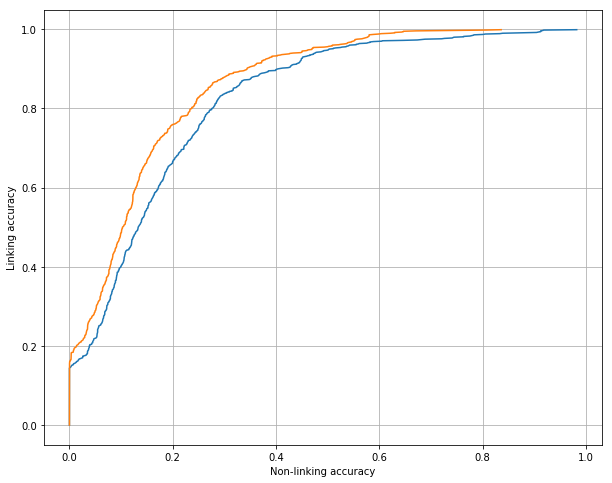
\includegraphics[width=0.7\textwidth]{graphics/linking2}
%		\caption{The $x$-axis represents accuracy of identifying a set of traces unlinked, and the $y$-axis represents the accuracy of the same set linked based on Equation~\ref{eq:link3}. Red is a link before, and blue is a link after.
%		\label{fig:linkcdf}}
%\end{center}\end{figure}